\documentclass[conference]{IEEEtran}
\IEEEoverridecommandlockouts
% The preceding line is only needed to identify funding in the first footnote. If that is unneeded, please comment it out.
\usepackage{cite}
\usepackage{amsmath,amssymb,amsfonts}
\usepackage{algorithmic}
\usepackage{graphicx}
\usepackage{textcomp}
\usepackage{xcolor}
\def\BibTeX{{\rm B\kern-.05em{\sc i\kern-.025em b}\kern-.08em
    T\kern-.1667em\lower.7ex\hbox{E}\kern-.125emX}}
\begin{document}

\title{TTDS CW3 Report\\
{A Search Engine to Explore ArXiv Abstracts}}


\author{authors}

\maketitle

\begin{abstract}
abstract here
\end{abstract}

\begin{IEEEkeywords}
BM25, TFIDF, Information Retrieval
\end{IEEEkeywords}

\section{Introduction}
Introduce the background of the project and the structure of the following sections.

\section{System Architecture Overview}
A whole view of the whole system.
\begin{figure}[h]
\centering
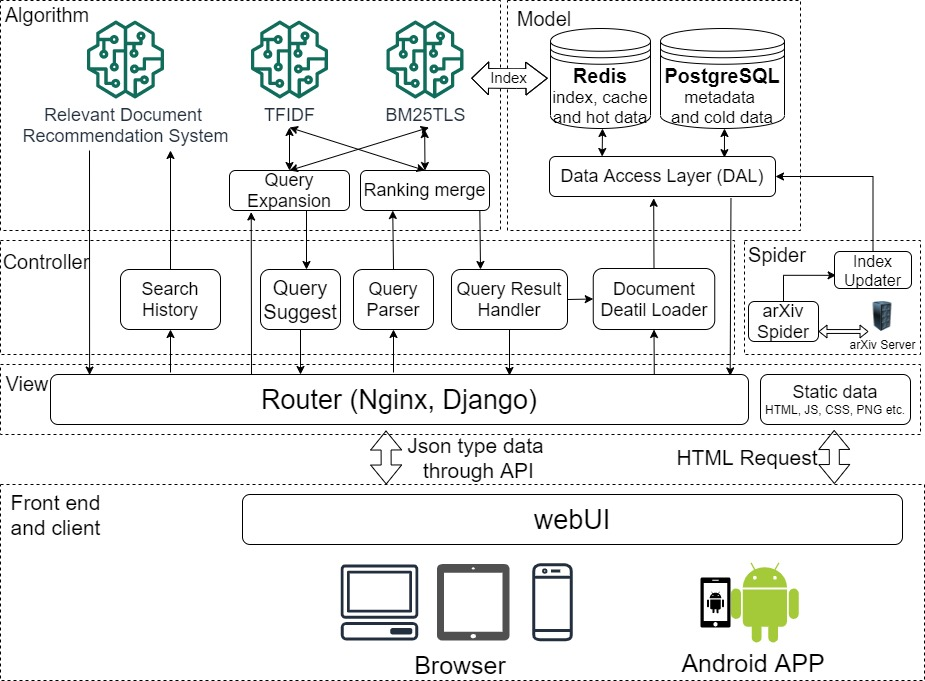
\includegraphics[width=3.5 in]{fig/structure} 
\caption{System Architecture}
\label{SystemArchitecture}
\end{figure}

\section{Data Format, Obtain, Preprocessing, Storage and Access}
\subsection{Data Format}

\subsection{Obtaining Raw Data}

\subsection{Preprocessing}

\subsection{Database Selection and Design}

\subsection{Data Access Layer}

\section{Indexing and Index Persistence}

\subsection{Index Structure}

\subsection{Index Persistence}

\subsection{Index Update}

\section{Retrieval Model and Algorithm}

\subsection{TFIDF}

\subsection{BM25TLS}

\subsection{Model Fusion}

\section{Implementation of Retrieval Model}

\subsection{Key Word Query}

\subsection{Query Expansion}

\subsection{Relative Document Recommendation}

\section{WebUI and Application}
\subsection{Web UI design}
\subsection{Android Application}

\section{Server Deployment and Performance Optimization}
\subsection{Server Deployment and Maintain}

\subsection{Performance Optimization}

\section{Highlight and Future work}



\end{document}
